
\chapter{Mapa 3D consistente en sistema prototipo}

\section{Filtrado de inconsistencias}
\label{sec:filtrado-estadistico-de-inconsistencias}

En el apartado \ref{sec:consideraciones-kinect}, se explica que el sensor Kinect no esta exento de error y que existen varias restricciones que pueden interferir en las mediciones de profundidad. Aplicando correctamente la técnica de medición digital presentada en la sección \ref{sec:metodologia-medicion-digital}, se disminuye la cantidad de datos incorrectos, pero no hay seguridad de eliminarlos completamente. Por otro lado, al finalizar un ensayo hidráulico, suele permanecer agua acumulada sobre la estructura del dique (con dificultad de drenar sin alterar la condición final del modelo) que puede generar mediciones espurias. \\ 
Con la motivación anterior, se decide aplicar una técnica de análisis estadístico presentada en \cite{Rusu08towards3d}, que busca eliminar mediciones incorrectas. Este enfoque se basa en el cómputo de la distribución de la distancias entre los puntos 3D. Para cada punto, el procedimiento calcula la media $\mu$ y la desviación estándar $\sigma$ de las distancias a sus \textsl{k} vecinos más cercanos. Asumiendo que la distribución resultante es normal $\mathcal{N}(\mu, \sigma^{2})$, todos los puntos que caen fuera del intervalo $\mu \pm \alpha \cdot \sigma$ pueden ser considerados \textit{outliers} y removidos del conjunto de datos. La figura \ref{fig:statistical-removal} muestra el efecto de la eliminación de \textit{outliers} sobre una nube de puntos 3D afectada por el ruido. \\ 
El valor de $\alpha$ depende del tamaño de la vecindad \textsl{k} analizada. En el presente trabajo, se utilizaron los valores $k=20, \alpha=2.5$, dando resultados satisfactorios, considerando aproximadamente 1\% de los puntos como \textit{outliers}.

\begin{figure}[ht]
\centering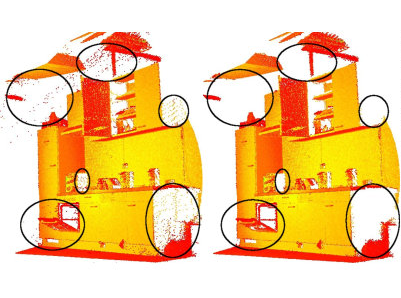
\includegraphics[width=\imsize]
{statistical-removal}
\caption[Eliminación de datos espurios con técnica estadística]
{Efectos del análisis estadístico y eliminación de outliers. Izquierda: la nube de puntos original. Derecha: resultado después de aplicar la técnica estadística \cite{Rusu08towards3d}.}
\label{fig:statistical-removal}
\end{figure}

\section{Mapa 3D en prototipo}
\label{sec:conversion-mapa3D-prototipo}

En ingeniería civil, para realizar estudios de variables sedimentológicas, los datos relevados sobre el modelo son referenciados con el sistema prototipo, es decir, se realiza una conversión a la escala natural de la obra y se define un sistema de coordenadas apropiado. Siguiendo estos lineamientos, se deriva un mapa 3D de la condición de erosión en sistema prototipo, a partir del mapa 3D obtenido en la etapa de registración.\\
En las figuras \ref{fig:sistema-modelo} y \ref{fig:sistema-prototipo} se ilustra una superficie observada desde diferentes sistemas de coordenadas. El sistema modelo (figura \ref{fig:sistema-modelo}) tiene su origen en la cámara Kinect (específicamente en la posición del sensor al iniciar la registración). Para poder realizar la conversión, se requiere asociar una cota (de altitud) en el sistema modelo a una cota en el sistema prototipo (figura \ref{fig:sistema-prototipo}), que defina consistentemente el nuevo sistema de coordenadas. \\ 
Además, se debe aplicar un re-escalado apropiado sobre la escena, debido a la reducción de escala propia de la modelización en laboratorio.\\
Para cada punto 3D $(x_{m}, y_{m}, z_{m})$ en el sistema modelo, la conversión a sistema prototipo $(x_{p}, y_{p}, z_{p})$ esta dada por:
\begin{equation}
x_{p} =   s \cdot x_{m}
\end{equation}
\begin{equation}
y_{p} = - s \cdot y_{m}
\end{equation}
\begin{equation}
z_{p} = - s \cdot (z_{p} - c_{m}) + c_{p}
\end{equation}
donde $c_{m}, c_{p}$ son las cotas de referencia para los sistema de coordenadas modelo y prototipo respectivamente, y \textsl{s} es la escala. \\

\begin{figure}[ht]
\centering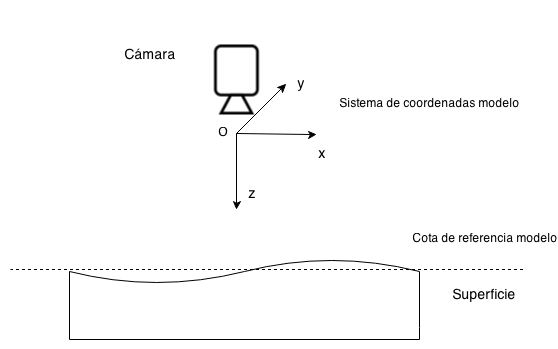
\includegraphics[width=\imsize]
{sistema-coordenadas-modelo}
\caption[Sistema de coordenadas modelo]
{Superficie desde sistema de coordenadas modelo.}
\label{fig:sistema-modelo}
\end{figure}

\begin{figure}[ht]
\centering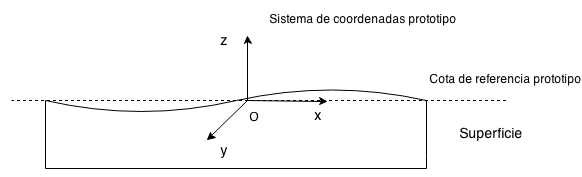
\includegraphics[width=\imsize]
{sistema-coordenadas-prototipo}
\caption[Sistema de coordenadas prototipo]
{Superficie desde sistema de coordenadas prototipo.}
\label{fig:sistema-prototipo}
\end{figure}

En el presente trabajo, la relación de escalas de longitudes modelo prototipo es $s=65$ (propiedad fijada en el modelo físico). La selección de las cotas de referencia varía dependiendo del área de interés en cada ensayo, utilizando siempre que fuera posible, cotas conocidas sobre la estructura del dique, provistas por estudios de topografía.
